\documentclass[12pt,a4paper,twocolumn]{article}
% The following LaTeX packages must be installed on your machine: amsmath, authblk, bm, booktabs, caption, dcolumn, fancyhdr, geometry, graphicx, hyperref, latexsym, natbib
\input{151.dat}
\usepackage{gensymb}
\usepackage{amsthm}
\usepackage{float}
\usepackage{siunitx}
\usepackage{amssymb}
\usepackage{float}
\usepackage{enumerate}
\usepackage{listings}
\usepackage{mathtools}
\PassOptionsToPackage{hyphens}{url}\usepackage{hyperref}
\usepackage[none]{hyphenat}
\usepackage{physics}
%\renewcommand{\familydefault}{\sfdefault}


\begin{document}

\setcounter{page}{1}

\section*{PS 33: Problem 3.43}
\bigskip

\begin{enumerate}[(a)]

\item The Lorentz distribution is given by

\begin{equation}\label{eq:lorentz}
	p(x) = \frac{1}{\pi}\frac{\gamma}{(x-a)^2 + \gamma^2}
\end{equation}

Comparing it with the Gaussian distribution:

\begin{figure}[!h]
	\centering
	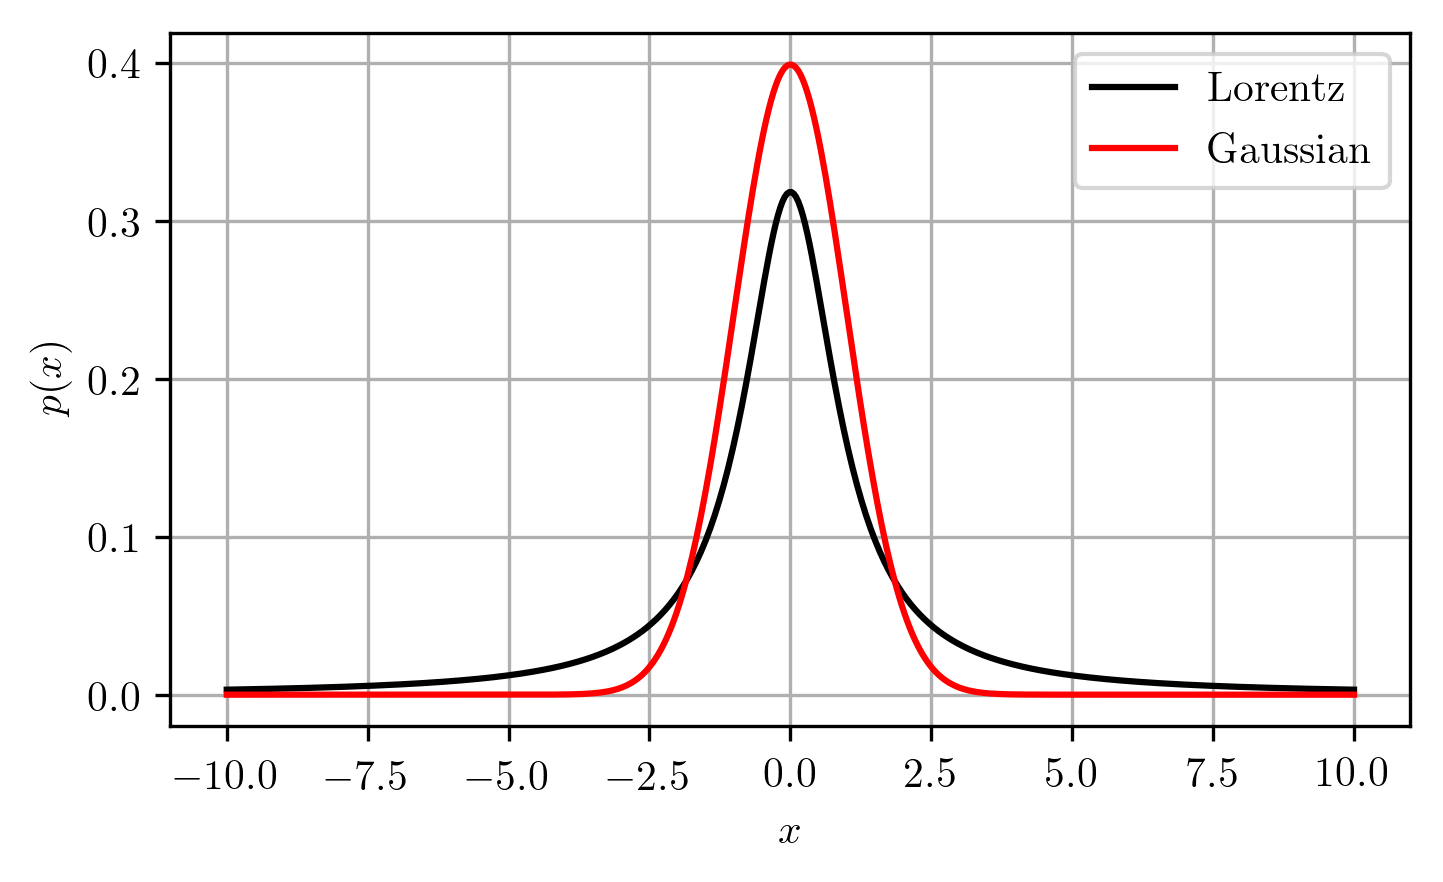
\includegraphics[width=\linewidth]{lorentz.png}
	\caption{Comparison of Lorentzian and Gaussian distributions.}
	\label{fig:compare}
\end{figure}

This shows that for the same set of parameters, the Gaussian has a higher peak, and quickly falls off and approaches zero as one moves away from the mean/central value.

\item For $a = 0$ and $\gamma = 1$, the first moment of the Lorentzian is given by

\begin{align}
	\ev{x^1} &= \int_{-\infty}^{+\infty} xp(x) \dd{x} \\
	&= \frac{1}{\pi} \int_{-\infty}^{+\infty} \frac{x}{x^2 + 1} \dd{x} \nonumber
\end{align}

Let $u \equiv x^2 + 1$, $\dd{u} \equiv 2x\dd{x}$,

\begin{align}
	\ev{x^1} &= \frac{1}{2\pi} \int_{-\infty}^{+\infty} \frac{1}{u}\dd{u} \nonumber \\
	&= \frac{1}{2\pi} \eval[\ln(u)|_{-\infty}^{+\infty} \nonumber \\
	&= \frac{1}{2\pi} \eval[\ln(x^2 + 1)|_{-\infty}^{+\infty} \nonumber
\end{align}

\end{enumerate}

\end{document}